\chapter{Pertukaran Gas Pernapasan}\label{ch:b1:gas-exchange}

Seliter udara memuat tiga puluh kali lebih banyak oksigen daripada
seliter air, berbobot delapan ratus kali lebih ringan, dan
membiarkan oksigen berdifusi melewatinya sepuluh ribu kali lebih
cepat. Seekor trout harus melewatkan seratus lima puluh gram air pada
\omterm{def:b1:gas-exchange:gill}{insangnya} bagi tiap miligram oksigen yang diambilnya, dan ia menyarikan
empat perlima dari yang dibawa airnya; seorang manusia menggerakkan
beberapa gram udara tiap miligram lalu menyia-nyiakan tiga
perempatnya. Kedua \omterm{def:b1:mammal-organization:organ}{organnya} adalah jawaban bagi persamaan yang sama
--- fluks sebuah gas melintasi sebuah permukaan --- dalam dua medium.
Bab ini menyatakan fisikanya, menurunkan apa yang harus dipenuhi
sebuah \omterm{prop:b1:organism-environment:surfaces}{permukaan pertukaran}, memerikan \omterm{def:b1:gas-exchange:gill}{insang}, \omterm{def:b1:gas-exchange:lung}{paru-paru} dan \omterm{def:b1:flowering-plant-organization:tissues}{trakea},
mengikuti oksigen dan karbon dioksida melalui darahnya, lalu menilik
bagaimana ventilasinya dikendalikan dan apa yang berubah di ketinggian
dan di bawah air.

\section{Fisika sebuah gas dalam dua medium}

\begin{definition}[Tekanan parsial, kelarutan]\label{def:b1:gas-exchange:partial}
\index{tekanan parsial}
Dalam sebuah campuran gas tiap gas mengerahkan sebuah \emph{tekanan
parsial} yang sebanding dengan fraksinya: dalam udara pada
\qty{101}{kPa}, oksigen (\qty{20.9}{\%}) memiliki
$P_{\mathrm{O_2}} = \qty{21.2}{kPa}$, karbon dioksida
(\qty{0.04}{\%}) \qty{0.04}{kPa}.
Sebuah gas larut dalam sebuah cairan sebanding dengan tekanan
parsialnya (hukum Henry): air yang setimbang dengan udara pada
\qty{15}{\celsius} memuat \qty{0.32}{mmol/L} oksigen (\qty{10}{mg/L},
\qty{7}{mL/L} gas), lawan \qty{8.7}{mmol/L} (\qty{210}{mL/L}) dalam
udaranya sendiri. Tekanan parsialnya --- sama dalam airnya dan
udaranya pada kesetimbangan --- itulah yang memacu difusi antarmedium;
kandungannya adalah apa yang dapat disarikan seorang pernapas. Karbon
dioksida dua puluh lima kali lebih larut daripada oksigen, sehingga ia
tak pernah menjadi gas yang lebih sukar dipertukarkan.
\end{definition}

\begin{theorem}[Hukum Fick bagi sebuah permukaan pertukaran]\label{thm:b1:gas-exchange:fick}
\index{hukum Fick}
Laju sebuah gas melintasi sebuah membran berluas $A$ dan bertebal $x$
yang memisahkan dua medium pada \omterm{def:b1:gas-exchange:partial}{tekanan parsial} $P_1$ dan $P_2$ adalah
\[
\dot V = K\,\frac{A}{x}\,(P_1 - P_2),
\]
dengan $K$, yaitu tetapan difusi (Krogh) membrannya, memadukan
kedifusian dan kelarutan gasnya dalam \omterm{def:b1:body-plans-tissues:tissue}{jaringannya}. Fluksnya dinaikkan
luas yang lebih besar, sawar yang lebih tipis dan beda \omterm{def:b1:gas-exchange:partial}{tekanan parsial}
yang lebih besar; tak ada yang lain.
\end{theorem}
\begin{proof}
Hukum pertama Fick bagi gas terlarut dalam membrannya
(\cref{ch:b1:membranes-transport}) memberikan fluks tiap satuan luas
yang sebanding dengan landaian kepekatannya; menurut hukum Henry
kepekatan pada tiap mukanya sebanding dengan \omterm{def:b1:gas-exchange:partial}{tekanan parsial} mediumnya
di sana, sehingga landaiannya adalah $(P_1 - P_2)/x$ kali kelarutannya,
dan tetapannya menyerap kelarutan dan kedifusiannya.
\end{proof}

\begin{omfigure}
\begin{tikzpicture}
\begin{axis}[
  ybar, bar width=16pt,
  width=0.72\linewidth, height=5.6cm,
  axis x line=bottom, axis y line=left,
  ymode=log, log origin=infty, ymin=0.1, ymax=3000,
  ylabel={oksigen tiap liter medium (\unit{mL})},
  ylabel style={font=\small},
  symbolic x coords={udara, air pada 5 C, air pada 15 C, air pada 30 C, air laut pada 15 C},
  xtick=data, x tick label style={font=\small, rotate=20, anchor=north east},
  enlarge x limits=0.15,
  nodes near coords, nodes near coords style={font=\scriptsize, anchor=south},
  point meta=rawy,
]
\addplot[fill=omDef!45, draw=omDef] coordinates {(udara,210) (air pada 5 C,9.0) (air pada 15 C,7.1) (air pada 30 C,5.3) (air laut pada 15 C,5.8)};
\end{axis}
\end{tikzpicture}

{\small Kandungan oksigen udara dan air yang setimbang dengannya. Air
memuat tiga puluh kali lebih sedikit, dan lebih sedikit lagi ketika
hangat atau asin: seekor ikan dalam kolam musim panas hidup di tepi
pasokannya.}
\end{omfigure}

\begin{proposition}[Apa yang harus dipenuhi sebuah permukaan pertukaran]\label{prop:b1:gas-exchange:requirements}
\index{permukaan pertukaran}
Sebuah \omterm{def:b1:organism-environment:organism}{organisme} yang lebih dari satu milimeter tak dapat dipasok
lewat difusi menembus permukaan luarnya
(\cref{ch:b1:organism-environment}). Ia memerlukan sebuah
\emph{permukaan pernapasan} yang luas (untuk menaikkan $A$), tipis
(untuk menurunkan $x$), lembap (gas melintasi membran hanya dalam
larutan), \emph{diventilasi} --- medium luarnya diperbarui, sehingga
$P_1$ tinggal tinggi --- dan \emph{diperfusi} --- darah di belakangnya
diperbarui, sehingga $P_2$ tinggal rendah; serta sebuah peredaran untuk
membawa gasnya dari permukaannya ke \omterm{def:b1:body-plans-tissues:tissue}{jaringannya}. \omterm{def:b1:gas-exchange:gill}{Insang}, \omterm{def:b1:gas-exchange:lung}{paru-paru} dan
\omterm{def:b1:flowering-plant-organization:tissues}{trakea} adalah tiga cara melipat permukaan semacam itu ke dalam sebuah
tubuh lalu menggerakkan kedua fluidanya melintasinya.
\end{proposition}

\section{Insang dan arus lawan}

\begin{definition}[Insang]\label{def:b1:gas-exchange:gill}
\index{insang}
Yang disebut \emph{insang} adalah evaginasi permukaan tubuh ke dalam
airnya, yang terlipat menjadi filamen dan \emph{lamela} setebal
beberapa mikrometer yang di dalamnya darah mengalir dalam kapiler.
Insang seekor ikan tergantung pada empat lengkung bertulang di tiap
sisinya; air yang ditarik masuk di mulutnya lalu didorong keluar di
bawah tutup insangnya oleh sebuah sistem dua pompa mengalir di antara
lamelanya pada satu arah, dan darah dalam lamelanya mengalir pada arah
yang lain: sebuah \emph{arus lawan}\index{pertukaran arus lawan}.
Seekor trout sekilogram memiliki sekitar \qty{2000}{cm^2} permukaan
lamela, setebal \qty{2}{\micro m}.
\end{definition}

\begin{omfigure}
\begin{tikzpicture}
  \node[anchor=south west, inner sep=0] (img) at (0,0)
    {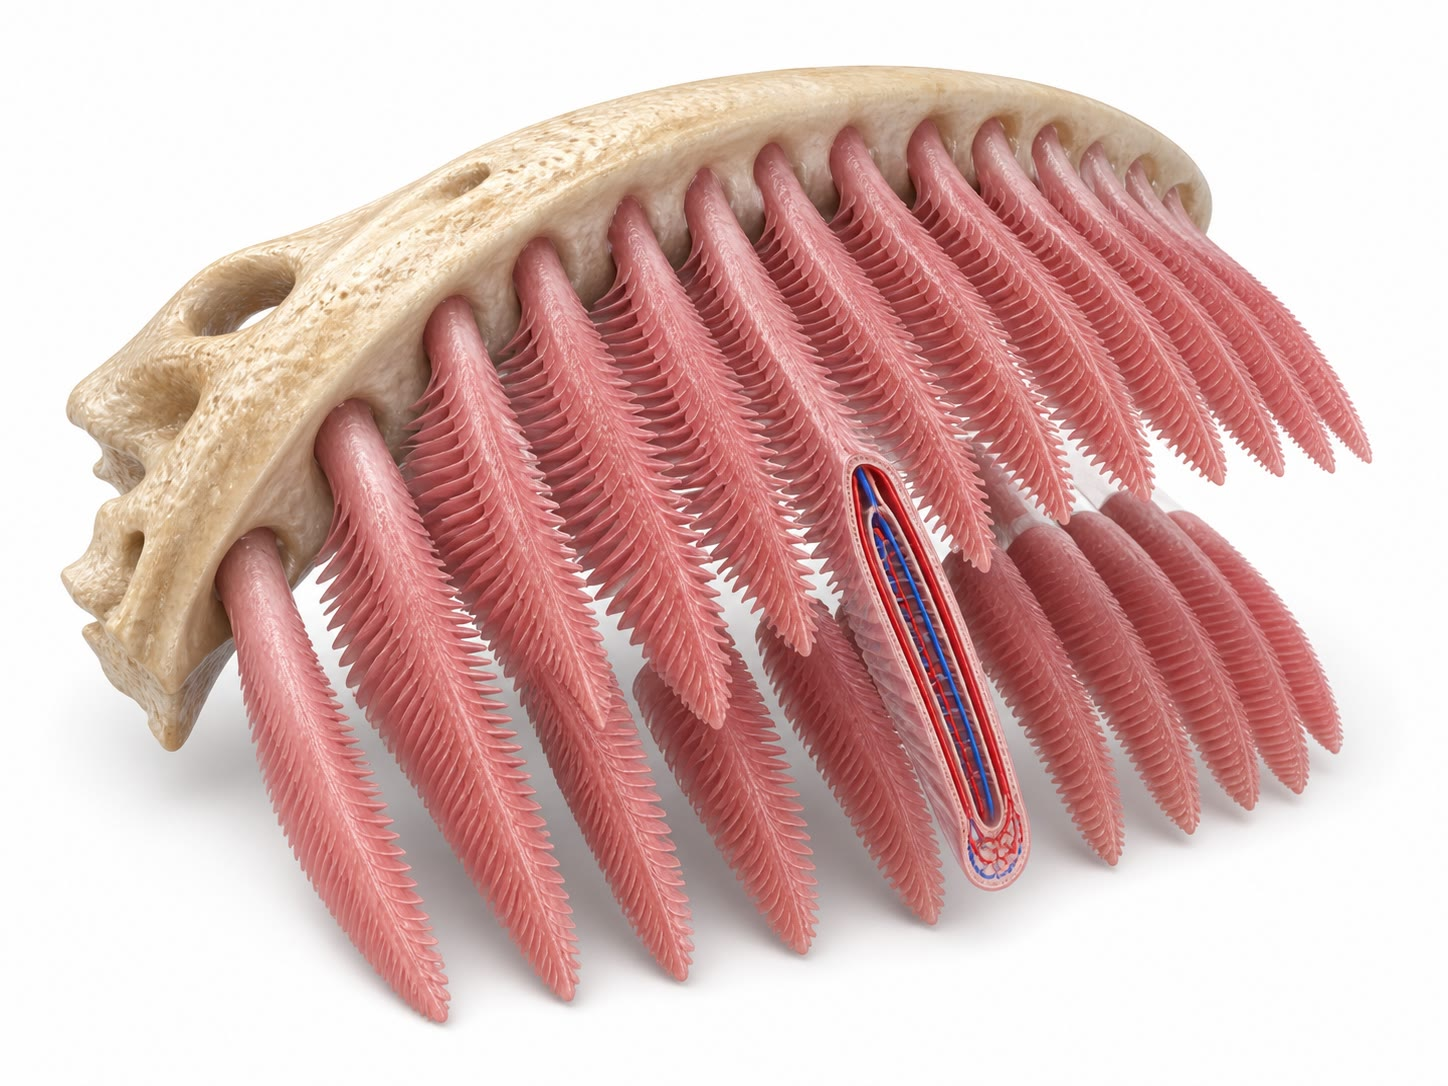
\includegraphics[width=0.52\linewidth]{images/book3/ai/fig-gill-lamellae.jpg}};
  \begin{scope}[x={(img.south east)}, y={(img.north west)},
      every node/.style={font=\small}]
    \draw[omDef, thick] (0.20,0.50) -- (-0.03,0.60) node[left] {lengkung insang};
    \draw[omDef, thick] (0.55,0.70) -- (0.55,1.08) node[above] {filamen};
    \draw[omDef, thick] (0.75,0.40) -- (1.03,0.30) node[right, align=left] {lamela: permukaan\\ pertukarannya, setebal \qty{2}{\micro m}};
    \draw[omDef, thick] (0.45,0.20) -- (0.45,-0.08) node[below] {pembuluh darah sepanjang filamennya};
  \end{scope}
\end{tikzpicture}

{\small Sebuah lengkung \omterm{def:b1:gas-exchange:gill}{insang} dengan filamen dan lamelanya. Air
mengalir di antara lamelanya; darah mengalir menembusnya pada arah
yang berlawanan.}
\end{omfigure}

\begin{theorem}[Pertukaran arus lawan]\label{thm:b1:gas-exchange:countercurrent}
Ketika air dan darah mengalir pada arah yang berlawanan sepanjang
sebuah \omterm{prop:b1:organism-environment:surfaces}{permukaan pertukaran}, darah yang meninggalkan \omterm{def:b1:gas-exchange:gill}{insangnya} dapat
mendekati \omterm{def:b1:gas-exchange:partial}{tekanan parsial} air yang \emph{memasukinya}, dan airnya dapat
dikuras hampir seluruh oksigennya: ekstraksi \qty{80}{\%} atau lebih.
Ketika keduanya mengalir pada arah yang sama (arus searah), kedua
fluidanya memusat ke sebuah nilai tengah bersama dan ekstraksinya tak
dapat melampaui \qty{50}{\%}.
\end{theorem}
\begin{proof}
Sepanjang sebuah penukar arus searah beda $P_{\text{air}} -
P_{\text{darah}}$ turun dari nilai masuknya ke nol seiring keduanya
mendekati tekanan yang sama; begitu keduanya setara tak ada lagi gas
yang berpindah, dan bagi laju alir yang setara titik temunya berada di
tengah. Dalam aliran \omterm{def:b1:gas-exchange:gill}{arus lawan} darahnya, seraya bergerak menuju
keluarnya, menemui air yang kian segar, sehingga sebuah beda yang
positif terpelihara sepanjang seluruh panjangnya; darah pada keluarnya
menghadapi air yang masuk pada \qty{21}{kPa}, dan air pada keluarnya
menghadapi darah vena yang masuk pada beberapa kilopascal. Batasnya
ditetapkan permukaannya, bukan sebuah kesetimbangan.
\end{proof}

\begin{omfigure}
\begin{tikzpicture}[font=\footnotesize, >=Stealth, line cap=round]
  % co-current
  \begin{scope}
    \node[anchor=south, font=\small] at (2.6,1.65) {arus searah: kedua aliran sehala};
    \draw[->, very thick, omDef] (0,1.2) -- (5.2,1.2) node[right] {air keluar: \qty{12}{kPa}};
    \draw[->, very thick, omThm] (0,0.4) -- (5.2,0.4) node[right] {darah keluar: \qty{12}{kPa}};
    \node[anchor=east, omDef] at (-0.1,1.2) {air masuk: \qty{21}{kPa}};
    \node[anchor=east, omThm] at (-0.1,0.4) {darah masuk: \qty{3}{kPa}};
    \foreach \x/\d in {0.6/18, 1.6/12, 2.6/7, 3.6/3, 4.6/0.5} { \draw[->, gray] (\x,1.05) -- (\x,0.55) node[midway, right, font=\scriptsize, gray] {\d}; }
    \node[anchor=north, align=center] at (2.6,0.1) {bedanya (kelabu, kPa) menyusut ke nol:\\ ekstraksinya berhenti pada \qty{43}{\%}};
  \end{scope}
  \begin{scope}[yshift=-3.6cm]
    \node[anchor=south, font=\small] at (2.6,1.65) {arus lawan: aliran berlawanan};
    \draw[->, very thick, omDef] (0,1.2) -- (5.2,1.2) node[right] {air keluar: \qty{4}{kPa}};
    \draw[<-, very thick, omThm] (0,0.4) -- (5.2,0.4) node[right] {darah masuk: \qty{3}{kPa}};
    \node[anchor=east, omDef] at (-0.1,1.2) {air masuk: \qty{21}{kPa}};
    \node[anchor=east, omThm] at (-0.1,0.4) {darah keluar: \qty{18}{kPa}};
    \foreach \x/\d in {0.6/3, 1.6/3, 2.6/3, 3.6/3, 4.6/2} { \draw[->, gray] (\x,1.05) -- (\x,0.55) node[midway, right, font=\scriptsize, gray] {\d}; }
    \node[anchor=north, align=center] at (2.6,0.1) {bedanya tetap positif sepanjang jalan:\\ ekstraksinya mencapai \qty{80}{\%}, darahnya pergi dekat nilai masuk airnya};
  \end{scope}
\end{tikzpicture}

{\small Pertukaran arus searah dan \omterm{def:b1:gas-exchange:gill}{arus lawan} dengan permukaan dan
laju alir yang sama. Melawankan alirannya memelihara sebuah landaian
sepanjang seluruh panjangnya lalu membiarkan darahnya mendekati tekanan
oksigen air yang segar.}
\end{omfigure}

\begin{omfigure}
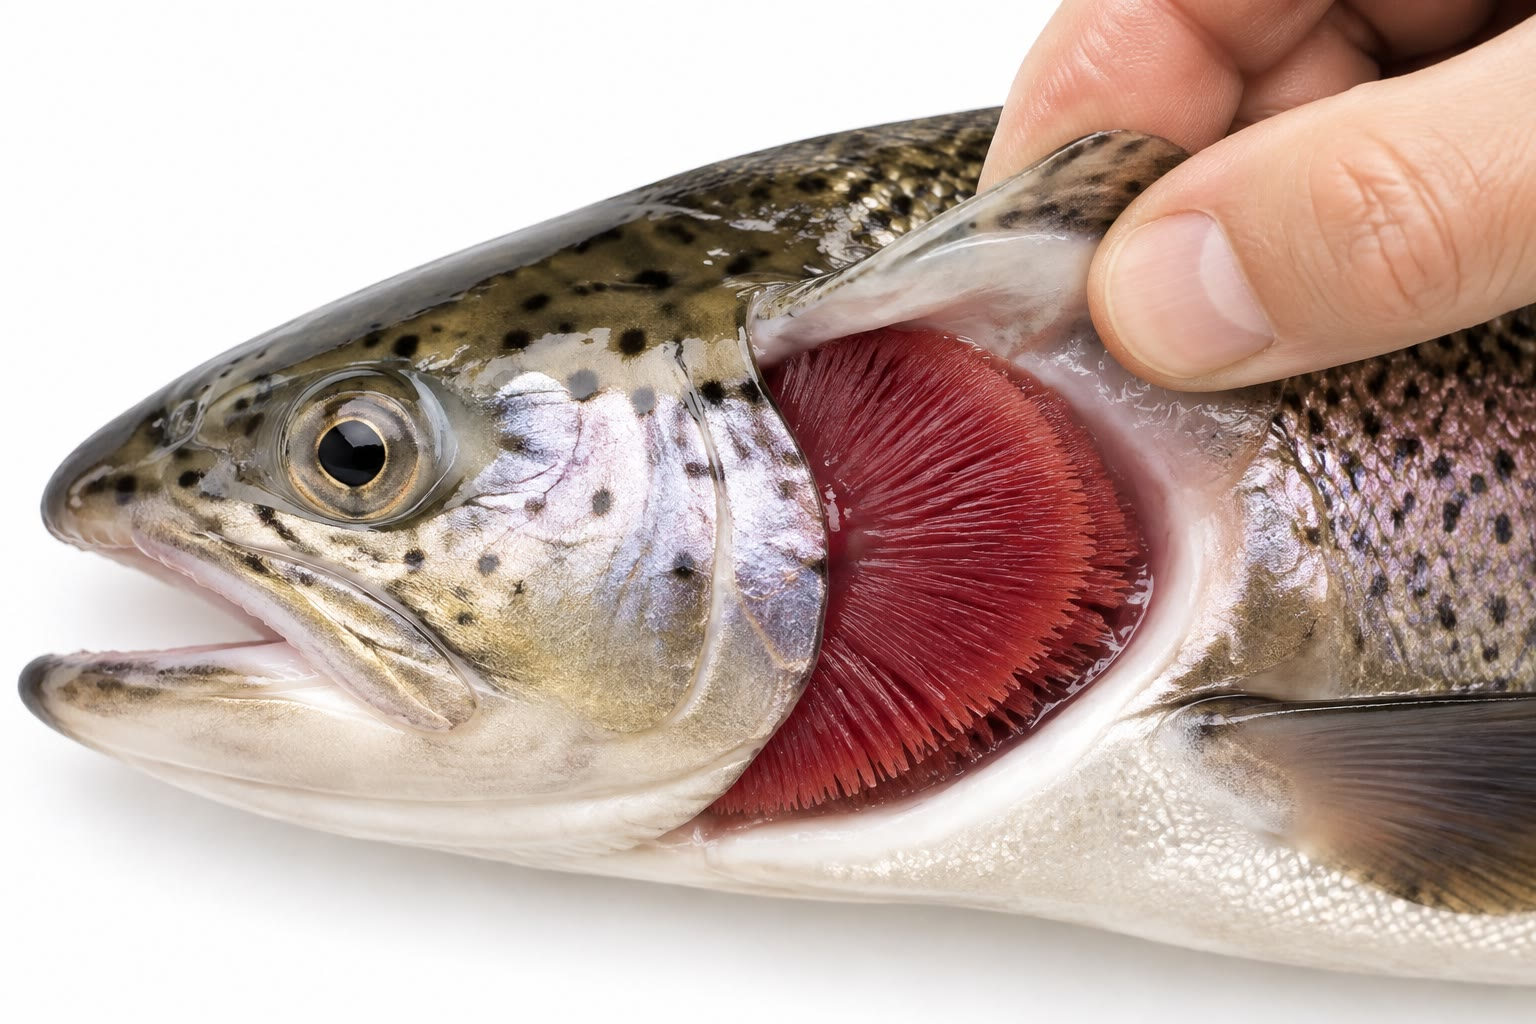
\includegraphics[width=0.5\linewidth]{images/book3/ai/b3-21-trout-gills.jpg}

{\small \omterm{def:b1:gas-exchange:gill}{Insang} seekor trout di bawah tutup \omterm{def:b1:gas-exchange:gill}{insang} yang terangkat:
merah oleh darahnya, sebab lamelanya setebal dua \omterm{def:b1:cell-unit-of-life:cell}{sel} dan darahnya
sejauh satu mikrometer dari airnya.}
\end{omfigure}

\begin{example}[Harga air]\label{ex:b1:gas-exchange:priceofwater}
Seekor trout istirahat seberat \qty{1}{kg} mengambil sekitar
\qty{50}{mL} oksigen sejam. Dari air pada \qty{7}{mL/L}, dengan
ekstraksi \qty{80}{\%}, ia harus memompa \qty{9}{L} air sejam melewati
\omterm{def:b1:gas-exchange:gill}{insangnya} --- sembilan kilogram sebuah medium yang lima puluh kali
lebih kental daripada udara, lewat saluran selebar sebagian kecil
milimeter. Sepersepuluh metabolismenya tersalur ke pernapasannya;
seorang manusia yang istirahat membelanjakan seperlima puluh. Hangatkan
kolamnya ke \qty{30}{\celsius} dan ikan yang sama, yang memerlukan
lebih banyak oksigen dari air yang memuat lebih sedikit, harus memompa
tiga kali lebih banyak.
\end{example}

\section{Bernapas dalam udara: paru-paru dan trakea}

\begin{definition}[Paru-paru mamalia]\label{def:b1:gas-exchange:lung}
\index{paru-paru}\index{alveolus}
Yang disebut \emph{paru-paru} adalah invaginasi permukaan tubuh ke
dalam sebuah ruang dalam yang lembap, yang menjaga permukaannya tetap
basah dalam udara kering. Paru-paru mamalia adalah sebuah pohon
saluran udara yang berakhir pada sekitar tiga ratus juta
\emph{alveolus}, yaitu kantung selebar \qty{0.2}{mm} yang dindingnya
--- satu \omterm{def:b1:cell-unit-of-life:cell}{sel} epitelium dan satu endotelium kapiler, \qty{0.5}{\micro m}
seluruhnya --- berjumlah \qty{100}{m^2} pada seorang manusia, terbungkus
sebuah jala kapiler yang dilewati seluruh curah jantungnya. Ia
diventilasi secara \emph{bolak-balik}: \omterm{def:b1:mammal-organization:bodyplan}{diafragma} dan otot iganya
\omterm{def:b1:cell-unit-of-life:resolution}{memperbesar} dadanya, udara mengalir masuk; keduanya mengendur, udara
mengalir keluar lewat jalan yang sama. Sekali napas menggerakkan
\qty{500}{mL}, yang \qty{150}{mL} di antaranya hanya mengisi saluran
udaranya (\emph{ruang mati}) lalu tak pernah mencapai sebuah alveolus;
gas alveolusnya, yang diperbarui sepertujuh pada tiap napas, tinggal
pada $P_{\mathrm{O_2}} =
\qty{13.3}{kPa}$ dan $P_{\mathrm{CO_2}} = \qty{5.3}{kPa}$ --- yakni
tekanan yang disetimbangi darahnya.
\end{definition}

\begin{omfigure}
\begin{tikzpicture}
  \node[anchor=south west, inner sep=0] (img) at (0,0)
    {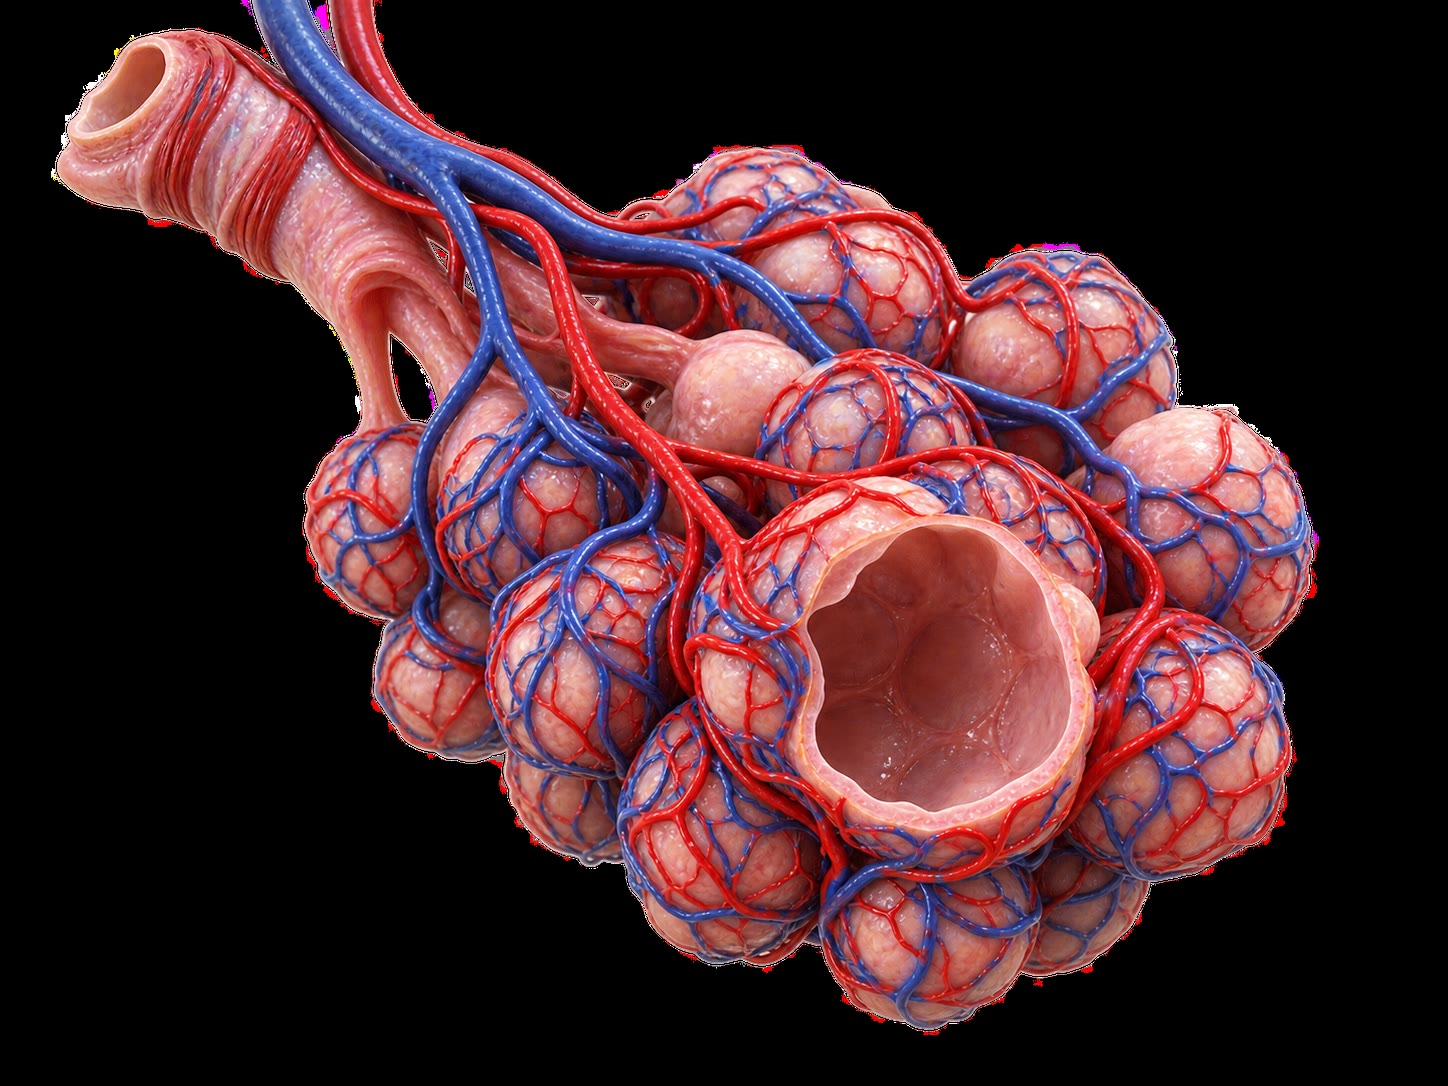
\includegraphics[width=0.5\linewidth]{images/book3/ai/fig-alveoli.jpg}};
  \begin{scope}[x={(img.south east)}, y={(img.north west)},
      every node/.style={font=\small}]
    \draw[omDef, thick] (0.50,0.85) -- (0.50,1.08) node[above] {saluran udara ujung};
    \draw[omDef, thick] (0.30,0.45) -- (-0.03,0.40) node[left, align=right] {alveolus yang dibelah:\\ udara di dalamnya};
    \draw[omDef, thick] (0.75,0.55) -- (1.03,0.62) node[right, align=left] {jala kapiler\\ pada dindingnya};
    \draw[omDef, thick] (0.60,0.15) -- (0.60,-0.08) node[below] {dinding: \qty{0.5}{\micro m} antara udara dan darah};
  \end{scope}
\end{tikzpicture}

{\small \omterm{def:b1:gas-exchange:lung}{Alveolus} pada ujung sebuah saluran udara, terbungkus kapiler.
Seluruh curah jantungnya menyebar pada seratus meter persegi dinding
ini, sepersekian sekon dalam satu kali.}
\end{omfigure}

\begin{proposition}[Tiga rancangan bagi udara]\label{prop:b1:gas-exchange:designs}
\index{trakea}
\emph{Mamalia} berventilasi secara bolak-balik: sederhana, tetapi
udara segarnya bercampur dengan yang basi, oksigen \omterm{def:b1:gas-exchange:lung}{alveolusnya} dua
pertiga oksigen atmosfernya, dan ekstraksinya seperempat.
\emph{Burung} melewatkan udara pada satu arah lewat tabung halus
(parabronkus) di antara dua perangkat kantung udara yang bertindak
sebagai puputan, sehingga udara segar mengalir menembus \omterm{prop:b1:organism-environment:surfaces}{permukaan
pertukarannya} baik pada tarikan maupun pada embusan napas, dalam
sebuah arus silang dengan darahnya: ekstraksinya lebih tinggi, dan
seekor angsa kepala palang terbang melintasi Himalaya tempat seekor
mamalia akan pingsan. \emph{Serangga} sama sekali tak memiliki darah
pernapasan: udara masuk lewat katup (\emph{spirakel}) ke dalam
\emph{\omterm{def:b1:flowering-plant-organization:tissues}{trakea}}, yaitu tabung yang dikakukan penebalan berpilin yang
bercabang sampai semikrometer lalu mengantarkan oksigen lewat difusi
langsung ke tiap \omterm{def:b1:cell-unit-of-life:cell}{selnya}, dibantu pemompaan perutnya pada serangga yang
besar atau giat. Difusi sepanjang tabung membatasi rancangannya pada
tubuh yang kecil --- yang menjadi salah satu sebab tak ada serangga
yang lebih besar daripada seekor tikus.
\end{proposition}

\begin{omfigure}
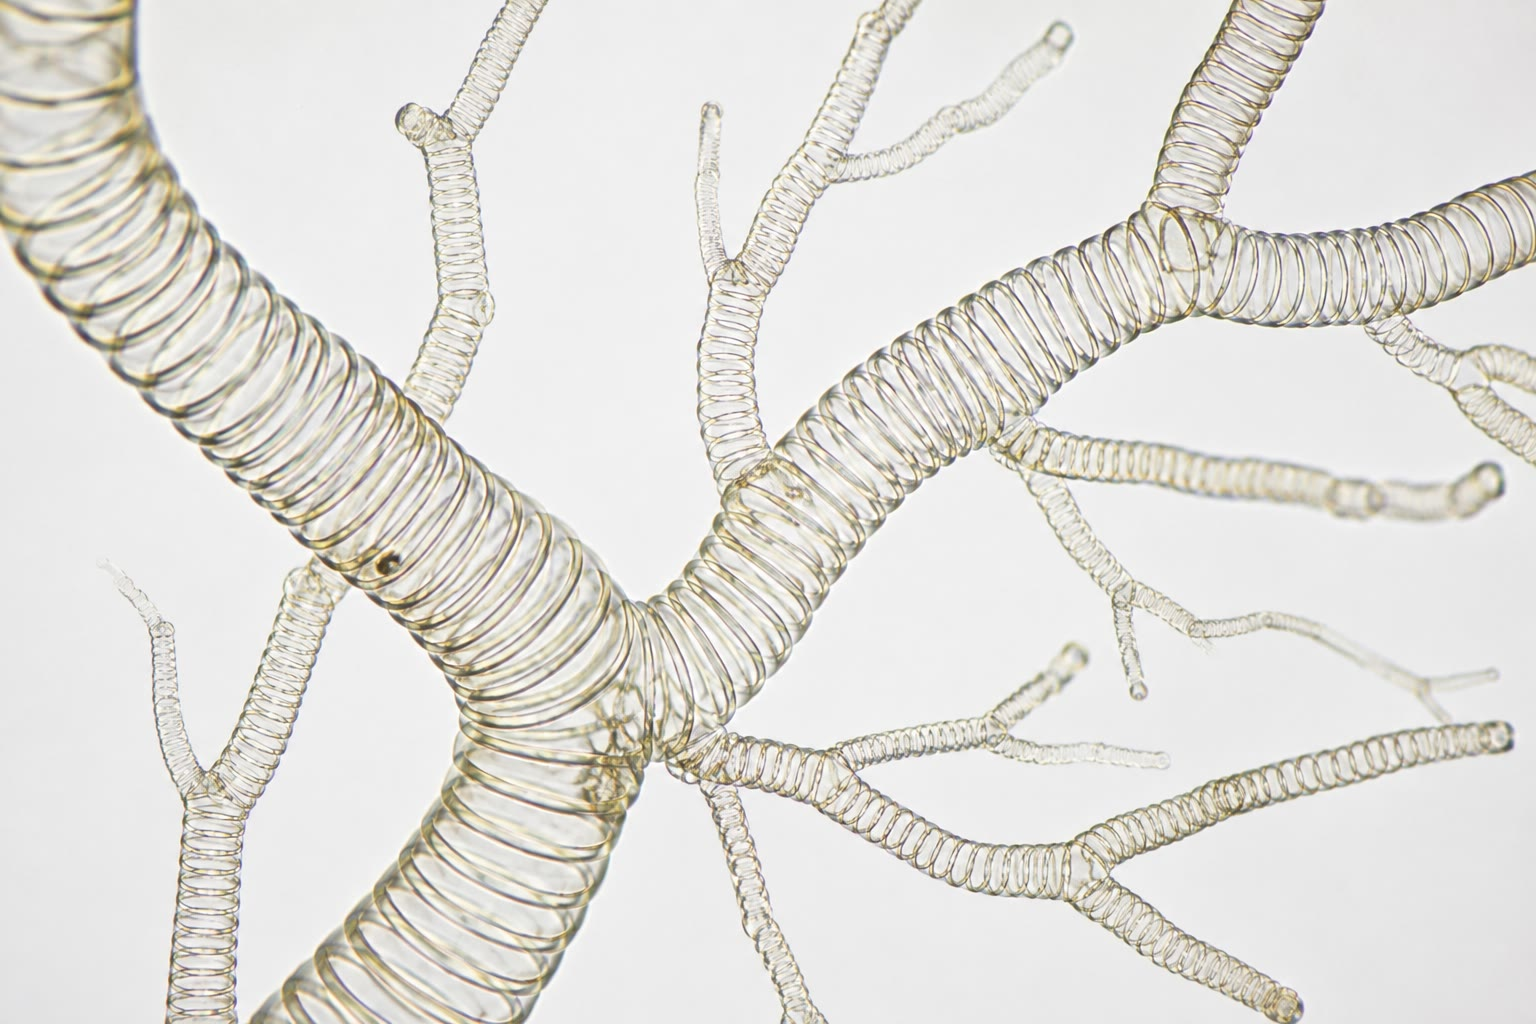
\includegraphics[width=0.5\linewidth]{images/book3/ai/b3-21-insect-tracheae.jpg}

{\small \omterm{def:b1:flowering-plant-organization:tissues}{Trakea} serangga: tabung berisi udara yang dijaga terbuka
penebalan berpilin, yang bercabang sampai ke \omterm{def:b1:cell-unit-of-life:cell}{selnya}. Tak ada darah
yang membawa oksigennya; udaranya menempuh seluruh jalannya.}
\end{omfigure}

\begin{method}[Membaca sebuah anggaran ventilasi]\label{met:b1:gas-exchange:budget}
\begin{enumerate}
  \item Ventilasi semenit $=$ volume tidal $\times$ napas tiap
        menit; ventilasi \omterm{def:b1:gas-exchange:lung}{alveolus} $=$ (volume tidal $-$ ruang mati)
        $\times$ napas tiap menit. Hanya yang kedua mempertukarkan gas.
  \item Serapan oksigen $=$ ventilasi \omterm{def:b1:gas-exchange:lung}{alveolus} $\times$ (fraksi
        terhirup $-$ fraksi \omterm{def:b1:gas-exchange:lung}{alveolus}); pada keadaan istirahat,
        $\qty{4.2}{L/min}\times(0.21 - 0.14) \approx \qty{0.3}{L/min}$.
  \item Ekstraksi $=$ serapan $/$ (ventilasi $\times$ fraksi
        terhirup): seperempat pada \omterm{def:b1:gas-exchange:lung}{paru-paru} bolak-balik, empat perlima
        pada \omterm{def:b1:gas-exchange:gill}{insang} \omterm{def:b1:gas-exchange:gill}{arus lawan}.
  \item Di sisi darahnya: serapan $=$ curah jantung $\times$
        (kandungan arteri $-$ vena); \qty{5}{L/min}$\times$
        \qty{50}{mL/L} pada keadaan istirahat, \qty{250}{mL/min} yang
        sama. Kedua anggarannya harus cocok.
\end{enumerate}
\end{method}

\section{Gas dalam darah}

\begin{proposition}[Pengangkutan oksigen dan karbon dioksida]\label{prop:b1:gas-exchange:transport}
\index{anhidrase karbonat}\index{efek Bohr}\index{efek Haldane}
Plasmanya melarutkan hanya \qty{3}{mL} oksigen tiap liter pada tekanan
arterinya; hemoglobin (\cref{ch:b1:proteins}) mengangkut \qty{200}{mL},
memuat di \omterm{def:b1:gas-exchange:lung}{paru-parunya} pada \qty{13.3}{kPa} lalu membongkar seperlima
sampai separuhnya di \omterm{def:b1:body-plans-tissues:tissue}{jaringannya}. Karbon dioksida menempuh tiga jalan:
\qty{7}{\%} terlarut, \qty{23}{\%} terikat pada gugus amina
hemoglobinnya, dan \qty{70}{\%} sebagai bikarbonat: dalam \omterm{def:b1:cell-unit-of-life:cell}{sel} merahnya,
\emph{\omterm{prop:b1:gas-exchange:transport}{anhidrase karbonat}} mengubah $\mathrm{CO_2}$ dan air menjadi asam
karbonat dalam beberapa milisekon, asamnya terurai, bikarbonatnya
meninggalkan \omterm{def:b1:cell-unit-of-life:cell}{selnya} sebagai tukaran klorida (\emph{pergeseran
klorida}), dan protonnya diambil hemoglobinnya. Kedua gasnya saling
menolong: asam dan $\mathrm{CO_2}$ menurunkan pertalian hemoglobin
terhadap oksigennya (\emph{\omterm{prop:b1:gas-exchange:transport}{efek Bohr}}), sehingga oksigennya dilepaskan
di tempat $\mathrm{CO_2}$ dibuat; dan hemoglobin yang terdeoksigenasi
mengikat proton dan $\mathrm{CO_2}$ lebih baik (\emph{\omterm{prop:b1:gas-exchange:transport}{efek Haldane}}),
sehingga $\mathrm{CO_2}$ diambil di tempat oksigennya dilepaskan, lalu
diserahkan di \omterm{def:b1:gas-exchange:lung}{paru-parunya} seiring oksigennya memuat.
\end{proposition}

\begin{omfigure}
\begin{tikzpicture}[font=\footnotesize, >=Stealth, line cap=round]
  % red cell
  \draw[very thick, omThm!80!black, fill=omThm!8, rounded corners=18pt] (0,0) rectangle (7.6,4.0);
  \node[anchor=north west, omThm!80!black, font=\small] at (0.15,3.95) {sel darah merah (dalam sebuah kapiler jaringan)};
  % CO2 in from tissue
  \draw[->, very thick, omDef] (-1.6,2.6) -- (0,2.6) node[pos=0, left, align=right] {$\mathrm{CO_2}$ dari\\ jaringannya};
  \node[draw, thick, fill=white, rounded corners=3pt, inner sep=2pt] (ca) at (2.0,2.6) {$\mathrm{CO_2} + \mathrm{H_2O} \to \mathrm{H_2CO_3}$};
  \node[anchor=south, font=\scriptsize, omProp!80!black] at (2.0,2.95) {anhidrase karbonat};
  \node[draw, thick, fill=white, rounded corners=3pt, inner sep=2pt] (dis) at (5.2,2.6) {$\mathrm{H^+} + \mathrm{HCO_3^-}$};
  \draw[->, thick] (ca) -- (dis);
  % bicarbonate out, chloride in
  \draw[->, very thick, omDef] (6.2,2.4) -- (6.2,0.9) -- (8.4,0.9) node[right, align=left] {$\mathrm{HCO_3^-}$ ke dalam plasmanya\\ (\qty{70}{\%} dari $\mathrm{CO_2}$-nya)};
  \draw[<-, very thick, gray] (6.9,1.85) -- (8.4,1.85) node[right, gray] {$\mathrm{Cl^-}$ sebagai tukarannya};
  % proton to Hb, O2 release
  \node[draw, thick, fill=omThm!25, rounded corners=3pt, inner sep=2pt] (hb) at (4.0,1.0) {hemoglobin};
  \draw[->, thick] (4.7,2.35) -- (4.2,1.3) node[midway, right, font=\scriptsize] {$\mathrm{H^+}$ terikat};
  \draw[->, very thick, omExo!70!black] (hb.west) -- (0,1.0) -- (-1.6,1.0) node[left, align=right] {$\mathrm{O_2}$ dilepaskan\\ (efek Bohr)};
  \node[anchor=north, align=center, gray] at (3.8,-0.2) {di paru-parunya tiap panah berbalik: oksigen memuat, proton dan $\mathrm{CO_2}$ dilepaskan,\\ bikarbonatnya masuk kembali ke selnya lalu $\mathrm{CO_2}$-nya diembuskan};
\end{tikzpicture}

{\small Karbon dioksida dalam sebuah \omterm{def:b1:cell-unit-of-life:cell}{sel} merah. \omterm{prop:b1:gas-exchange:transport}{Anhidrase karbonat}
membuat asam karbonat; bikarbonatnya pergi ke plasmanya dan protonnya
diambil hemoglobinnya, yang melepaskan oksigen seraya mengikatnya.}
\end{omfigure}

\begin{example}[Seliter darah melewati sebuah otot yang bekerja]\label{ex:b1:gas-exchange:litre}
Darah arteri membawa \qty{200}{mL} oksigen tiap liter dan
\qty{480}{mL} karbon dioksida (sebagian besarnya sebagai bikarbonat).
Dalam sebuah otot yang istirahat ia meninggalkan \qty{50}{mL} oksigen
lalu mengambil \qty{40}{mL} $\mathrm{CO_2}$; pH venanya turun hanya
\qty{0.04}{}, sebab hemoglobinnya telah menyerap protonnya. Dalam
sebuah otot yang berlari cepat, pada pH 7,2 dan $P_{\mathrm{O_2}}$
sebesar \qty{2.7}{kPa}, liter yang sama meninggalkan \qty{150}{mL}
oksigen (\cref{ch:b1:proteins}) lalu membawa pergi laktatnya pula.
\end{example}

\section{Kendali, ketinggian dan penyelaman}

\begin{proposition}[Ventilasinya dikendalikan karbon dioksida]\label{prop:b1:gas-exchange:control}
\index{kemoreseptor}
Irama napasnya dibangkitkan dalam batang otaknya lalu disetel
\emph{kemoreseptor}: yang di pusat, yang terendam cairan di sekeliling
otaknya, menanggapi perubahan pH yang dihasilkan $\mathrm{CO_2}$; yang
di tepi dalam arteri karotisnya menanggapi turunnya oksigen arteri di
bawah sekitar \qty{8}{kPa}. Dalam kehidupan biasa
$\mathrm{CO_2}$-lah yang berkuasa: naiknya \qty{1}{kPa} pada
$P_{\mathrm{CO_2}}$ arterinya kira-kira melipatduakan ventilasinya,
sedangkan oksigennya harus turun sepertiga sebelum ventilasinya
menanggapi. Menahan napas berakhir ketika $\mathrm{CO_2}$, bukan
oksigennya, mencapai batasnya; bernapas berlebihan lebih dahulu
menurunkan $\mathrm{CO_2}$ lalu membiarkan seorang penyelam bertahan di
bawah sampai oksigennya habis --- pingsan sebelum dorongan bernapasnya
kembali.
\end{proposition}

\begin{omfigure}
\begin{tikzpicture}
\begin{axis}[
  width=0.86\linewidth, height=5.8cm,
  axis x line=bottom, axis y line=left,
  xmin=4, xmax=8.5, ymin=0, ymax=45,
  xlabel={$P_{\mathrm{CO_2}}$ arteri (\unit{kPa})}, ylabel={ventilasi (\unit{L/min})},
  xlabel style={font=\small, at={(axis description cs:0.5,-0.13)}, anchor=north},
  ylabel style={font=\small},
  tick label style={font=\small}, xtick={4,5,6,7,8}, ytick={0,10,20,30,40},
  legend style={font=\small, at={(0.03,0.97)}, anchor=north west, draw=none},
  clip=false,
]
\addplot[very thick, omDef, domain=4.5:8.5, samples=20] {6 + 10*(x-5.3)};
\addlegendentry{oksigen normal}
\addplot[very thick, omThm, domain=4.5:7.2, samples=20] {6 + 20*(x-5.3)};
\addlegendentry{oksigen rendah (\qty{7}{kPa}): lebih curam}
\draw[dashed, gray] (axis cs:5.3,0) -- (axis cs:5.3,6); \node[font=\scriptsize, anchor=west] at (axis cs:5.4,1.5) {nilai istirahatnya};
\end{axis}
\end{tikzpicture}

{\small Ventilasi lawan karbon dioksida arteri. Tiap kilopascal di
atas nilai istirahatnya menambahkan sekitar \qty{10}{L/min}; oksigen
yang rendah membuat tanggapannya lebih curam tetapi, sendirian, sedikit
berbuat sampai ia parah.}
\end{omfigure}

\begin{example}[Ketinggian dan kedalaman]\label{ex:b1:gas-exchange:altitudediving}
Pada \qty{4000}{m} udaranya memuat \qty{12}{kPa} oksigen dan
\omterm{def:b1:gas-exchange:lung}{alveolusnya} \qty{7}{}: badan karotisnya memacu ventilasinya naik, yang
mengembuskan $\mathrm{CO_2}$ lalu membuat darahnya basa --- sebuah rem
yang dilepaskan ginjalnya selama beberapa hari dengan mengeluarkan
bikarbonat; \omterm{def:b1:cell-unit-of-life:cell}{sel} merahnya menaikkan BPG-nya dalam beberapa hari dan
sumsumnya menaikkan hemoglobinnya dalam beberapa pekan
(\cref{ch:b1:proteins}). Seekor anjing laut yang menyelam selama dua
puluh menit berbuat sebaliknya: ia mengembuskan napas sebelum
menyelam, memperlambat jantungnya menjadi sepersepuluh, menutup
darahnya dari segalanya kecuali otak dan jantungnya, lalu menjalankan
ototnya dengan oksigen yang terikat pada mioglobinnya sendiri, sepuluh
kali lebih pekat daripada milik kita, lalu dengan \omterm{def:b1:respiration-fermentation:fermentation}{fermentasi}, sambil
menoleransi laktat yang dibersihkan tubuhnya di permukaan.
\omterm{def:b1:gas-exchange:lung}{Paru-parunya} kempis di bawah \qty{50}{m}, yang menjaga nitrogen tetap
di luar darahnya.
\end{example}

\section{Latihan}

\begin{exercise}[$\star$]\label{exo:b1:gas-exchange:1}
Nyatakan \omterm{thm:b1:membranes-transport:fick}{hukum Fick} bagi sebuah \omterm{prop:b1:organism-environment:surfaces}{permukaan pertukaran} lalu sebutkan
keempat ciri yang menaikkan fluksnya.
\end{exercise}

\begin{exercise}[$\star$]\label{exo:b1:gas-exchange:2}
Jelaskan mengapa air adalah medium yang lebih sukar dinapasi daripada
udara, dengan tiga angka.
\end{exercise}

\begin{exercise}[$\star$]\label{exo:b1:gas-exchange:3}
Dari gambar \omterm{def:b1:gas-exchange:gill}{arus lawannya}, bacalah tekanan oksigen air yang pergi dan
darah yang pergi pada tiap susunannya, serta ekstraksinya.
\end{exercise}

\begin{exercise}[$\star$]\label{exo:b1:gas-exchange:4}
Dalam tiga bentuk apakah karbon dioksida diangkut dalam darahnya, dan
dalam nisbah berapa?
\end{exercise}

\begin{exercise}[$\star\star$]\label{exo:b1:gas-exchange:5}
Seseorang bernapas \qty{15}{} kali semenit dengan volume tidal
\qty{450}{mL} dan ruang mati \qty{150}{mL}. Hitunglah ventilasi semenit
dan ventilasi \omterm{def:b1:gas-exchange:lung}{alveolusnya} serta serapan oksigennya bila fraksi
\omterm{def:b1:gas-exchange:lung}{alveolusnya} \qty{14}{\%}. Ulangi bagi \qty{30}{} napas dangkal sebesar
\qty{225}{mL}.
\end{exercise}

\begin{exercise}[$\star\star$]\label{exo:b1:gas-exchange:6}
Sebuah akuarium ikan mas pada \qty{25}{\celsius} memuat \qty{6}{mL}
oksigen tiap liter. Seekor ikan seberat \qty{20}{g} memakai \qty{2}{mL}
oksigen sejam. Berapa banyak air yang harus melintasi \omterm{def:b1:gas-exchange:gill}{insangnya} tiap
jam pada ekstraksi \qty{75}{\%}, dan berapa kali volumenya sendiri
itu?
\end{exercise}

\begin{exercise}[$\star\star$]\label{exo:b1:gas-exchange:7}
Sebuah \omterm{def:b1:gas-exchange:lung}{paru-paru} seluas \qty{100}{m^2} dan setebal \qty{0.5}{\micro m}
memindahkan \qty{250}{mL/min} pada beda tekanan purata \qty{8}{kPa}.
Sebuah penyakit menebalkan dindingnya menjadi \qty{2}{\micro m} lalu
memperkecil luasnya menjadi separuh. Hitunglah pemindahannya pada beda
yang sama, dan beda yang dibutuhkan untuk memulihkan \qty{250}{mL/min}.
Mengapa tubuhnya tak dapat sekadar menaikkan bedanya?
\end{exercise}

\begin{exercise}[$\star\star$]\label{exo:b1:gas-exchange:8}
Jelaskan pergeseran kloridanya: mengapa bikarbonatnya meninggalkan \omterm{def:b1:cell-unit-of-life:cell}{sel}
merahnya, mengapa kloridanya masuk, dan apa yang akan terjadi pada
volume \omterm{def:b1:cell-unit-of-life:cell}{selnya} tanpa pertukaran itu.
\end{exercise}

\begin{exercise}[$\star\star$]\label{exo:b1:gas-exchange:9}
Mengapa seorang penyelam yang bernapas berlebihan sebelum menyelam
sambil menahan napas berisiko tenggelam, sedangkan yang tidak
melakukannya muncul dengan selamat, tak nyaman tetapi sadar?
\end{exercise}

\begin{exercise}[$\star\star\star$]\label{exo:b1:gas-exchange:10}
Sebuah \omterm{def:b1:flowering-plant-organization:tissues}{trakea} serangga sepanjang \qty{1}{mm} dan selebar
\qty{20}{\micro m} memasok sebuah otot yang memakai \qty{1e-9}{mol}
oksigen tiap sekon. Dengan $D = \qty{2e-5}{m^2/s}$ dalam udara dan
\qty{8.7}{mol/m^3} oksigen pada spirakelnya, hitunglah kepekatannya
pada ujung ototnya (Fick: $J = DA\,\Delta c/L$). Ulangi bagi sebuah
\omterm{def:b1:flowering-plant-organization:tissues}{trakea} sepanjang \qty{10}{mm}. Apa yang membatasi ukuran serangga?
\end{exercise}

\begin{exercise}[$\star\star\star$]\label{exo:b1:gas-exchange:11}
Burung dan ikan sama-sama memakai aliran yang tidak bolak-balik.
Bandingkan penukarnya (arah mediumnya, hubungannya dengan aliran
darahnya, ekstraksinya) lalu jelaskan mengapa sebuah \omterm{def:b1:gas-exchange:lung}{paru-paru}
bolak-balik tak dapat mencapai ekstraksi keduanya berapa pun
permukaannya.
\end{exercise}

\begin{exercise}[$\star\star\star$]\label{exo:b1:gas-exchange:12}
``\omterm{def:b1:gas-exchange:lung}{Paru-paru} diatur oleh gas yang dikeluarkannya, bukan oleh gas yang
diambilnya.'' Bahaslah dalam satu paragraf: mengapa $\mathrm{CO_2}$
menjadi isyarat yang lebih baik di paras laut, kapan susunannya gagal,
dan bagaimana ketinggian menyingkapkannya.
\end{exercise}

\section{Soal: Seekor Trout dan Seorang Manusia}

\begin{problem}[{Soal akhir pekan --- sebuah insang dan sebuah
paru-paru yang disandingkan: oksigen tiap liter medium, ventilasi dan
ekstraksi, aliran arus lawan dan bolak-balik, serta darah di belakang
masing-masing, berakhir pada dayaguna ekstraksi insang arus lawannya}]
\label{pb:b1:gas-exchange:1}
Seorang manusia yang istirahat mengambil \qty{250}{mL} oksigen semenit,
bernapas \qty{12}{} kali semenit dengan volume tidal \qty{500}{mL} dan
ruang mati \qty{150}{mL}; udara terhirupnya \qty{21}{\%} oksigen, gas
\omterm{def:b1:gas-exchange:lung}{alveolusnya} \qty{14}{\%}; curah jantungnya \qty{5}{L/min}, kandungan
oksigen arterinya \qty{200}{mL/L}. Seekor trout istirahat seberat
\qty{1}{kg} mengambil \qty{50}{mL} oksigen sejam dalam air pada
\qty{15}{\celsius} yang memuat \qty{7}{mL/L}; hemoglobinnya mengangkut
\qty{100}{mL/L} ketika \omterm{def:b1:lipids:fattyacid}{jenuh}; darahnya meninggalkan \omterm{def:b1:gas-exchange:gill}{insangnya}
\qty{95}{\%} \omterm{def:b1:lipids:fattyacid}{jenuh} lalu kembali \qty{15}{\%} \omterm{def:b1:lipids:fattyacid}{jenuh}. Air \qty{800}{}
kali lebih rapat daripada udara.

\medskip
\noindent\textbf{Bagian I --- Dua medium.}
\begin{enumerate}
  \item Nyatakan kandungan oksigen udara dan air troutnya dalam
        milimol tiap liter (\qty{22.4}{L/mol}).
  \item Hitunglah nisbah kedua kandungannya.
  \item Hitunglah massa medium (udara \qty{1.2}{g/L}; air
        \qty{1000}{g/L}) yang memuat \qty{1}{mmol} oksigen pada tiap
        halnya.
  \item Hitunglah volume air troutnya yang memuat oksigen sebanyak
        seliter udara.
  \item Jelaskan dalam satu kalimat mengapa \omterm{def:b1:gas-exchange:gill}{insang} ikan harus
        diventilasi pada satu arah sedangkan \omterm{def:b1:gas-exchange:lung}{paru-paru} boleh
        bolak-balik.
\end{enumerate}

\medskip
\noindent\textbf{Bagian II --- \omterm{def:b1:gas-exchange:lung}{Paru-parunya}.}
\begin{enumerate}[resume]
  \item Hitunglah ventilasi semenit dan ventilasi \omterm{def:b1:gas-exchange:lung}{alveolusnya}.
  \item Berapa fraksi tiap napasnya yang berupa ruang mati, dan berapa
        fraksi ventilasi semenitnya yang karena itu terbuang?
  \item Hitunglah oksigen yang diantarkan ke \omterm{def:b1:gas-exchange:lung}{alveolusnya} tiap menit
        dan oksigen yang diserap (ventilasi \omterm{def:b1:gas-exchange:lung}{alveolus} $\times$ beda
        fraksinya). Periksalah terhadap \qty{250}{mL/min}.
  \item Hitunglah dayaguna ekstraksinya: serapan dibagi oksigen dalam
        ventilasi semenit yang terhirup.
  \item Hitunglah $P_{\mathrm{O_2}}$ \omterm{def:b1:gas-exchange:lung}{alveolusnya} dari fraksi
        \omterm{def:b1:gas-exchange:lung}{alveolusnya} (tekanan total \qty{101}{kPa}, uap air
        \qty{6.3}{kPa} yang harus dikurangkan lebih dahulu).
  \item Di sisi darahnya, hitunglah beda arteri-vena yang dibutuhkan
        bagi \qty{250}{mL/min} pada \qty{5}{L/min}, serta kandungan dan
        kejenuhan venanya.
  \item Selama olahraga serapannya naik menjadi \qty{3}{L/min} dengan
        curah jantung \qty{20}{L/min}. Hitunglah beda arteri-vena dan
        kejenuhan venanya.
\end{enumerate}

\medskip
\noindent\textbf{Bagian III --- \omterm{def:b1:gas-exchange:gill}{Insangnya}.}
\begin{enumerate}[resume]
  \item Hitunglah serapan oksigen troutnya dalam mililiter tiap menit.
  \item Dengan ekstraksi \qty{80}{\%} (\omterm{def:b1:gas-exchange:gill}{arus lawan}), hitunglah air yang
        diventilasi tiap menit dan tiap jam.
  \item Dengan ekstraksi yang akan diberikan sebuah penukar arus
        searah berpermukaan sama (\qty{43}{\%}), hitunglah air yang
        dibutuhkan. Apa yang dihemat \omterm{def:b1:gas-exchange:gill}{arus lawannya}?
  \item Hitunglah massa air yang dipompa tiap jam, lalu bandingkanlah
        dengan massa udara yang digerakkan seorang manusia tiap jam.
  \item Hitunglah beda arteri-vena troutnya dalam kandungan oksigen
        serta curah jantung yang dituntut serapannya.
  \item Hitunglah nisbah alir air terhadap alir darah pada \omterm{def:b1:gas-exchange:gill}{insangnya},
        dan nisbah alir udara terhadap alir darah pada \omterm{def:b1:gas-exchange:lung}{paru-paru}
        manusianya (ventilasi \omterm{def:b1:gas-exchange:lung}{alveolus} dibagi curah jantung).
        Berilah ulasan.
  \item Memompa air memakan biaya sekitar \qty{10}{\%} serapan oksigen
        troutnya. Bila airnya menghangat ke \qty{25}{\celsius}
        (\qty{5.5}{mL/L}) dan serapannya naik setengah, berapa kali
        ventilasinya harus naik, dan apa yang terjadi pada fraksi yang
        dibelanjakan untuk bernapas?
\end{enumerate}

\medskip
\noindent\textbf{Bagian IV --- Penukarnya sendiri.}
\begin{enumerate}[resume]
  \item Dalam \omterm{def:b1:gas-exchange:gill}{insang} \omterm{def:b1:gas-exchange:gill}{arus lawannya} darah pergi pada \qty{18}{kPa}
        sambil menghadapi air yang masuk pada \qty{21}{kPa}, dan air
        pergi pada \qty{4}{kPa} sambil menghadapi darah yang masuk pada
        \qty{3}{kPa}. Hitunglah beda tekanan pada tiap ujungnya.
  \item Dalam sebuah penukar arus searah kedua fluidanya pergi pada
        \qty{12}{kPa}. Hitunglah bedanya pada tiap ujungnya lalu
        jelaskan mengapa pertukarannya berhenti sebelum airnya
        terpakai habis.
  \item \omterm{def:b1:gas-exchange:lung}{Paru-paru} manusianya: \omterm{def:b1:gas-exchange:lung}{alveolusnya} \qty{13.3}{kPa}, darah vena
        yang tiba pada \qty{5.3}{kPa}, arteri yang pergi pada
        \qty{13.3}{kPa}. Susunan yang mana yang menyerupai sebuah
        \omterm{def:b1:gas-exchange:lung}{paru-paru} bolak-balik, dan mengapa darah arterinya tak dapat
        melampaui nilai \omterm{def:b1:gas-exchange:lung}{alveolusnya}?
  \item Lamela seekor trout berjumlah \qty{2000}{cm^2} pada tebal
        \qty{2}{\micro m}; \omterm{def:b1:gas-exchange:lung}{alveolus} seorang manusia \qty{100}{m^2} pada
        \qty{0.5}{\micro m}. Hitunglah nisbah $A/x$ keduanya, dan
        nisbah serapan oksigennya. Apa yang disiratkan perbandingannya
        tentang beda tekanan purata melintasi sebuah lamela relatif
        terhadap sebuah dinding \omterm{def:b1:gas-exchange:lung}{alveolus}?
  \item Jelaskan mengapa karbon dioksida tak pernah membatasi seekor
        ikan walaupun airnya memuat begitu sedikit oksigen.
  \item Nyatakan hasilnya: dayaguna ekstraksi \omterm{def:b1:gas-exchange:gill}{insang} troutnya dan
        \omterm{def:b1:gas-exchange:lung}{paru-paru} manusianya, serta kedua ciri \omterm{def:b1:gas-exchange:gill}{insangnya} yang membuat
        perbedaannya.
\end{enumerate}
\end{problem}
